\usetikzlibrary{shadings,shadows,shapes.arrows}

\begin{tikzpicture}
	\tikzstyle{blockstyle} = [draw,drop shadow,outer sep=3,inner sep=7,minimum size=57,line width=1, thin, draw=black!55, top color=white,bottom color=cyan]
	\def\k{1}
	\node (A) at (0,3*\k) {$\cfrac{\partial e}{\partial d_1}(-1,2)$};
	\node[blockstyle] (B) at (0,0*\k) {$d_1$};
	\node (C) at (0,-3*\k) {$\cfrac{de}{dc}(4)$};
	
	\path[->] (A) edge node [right,xshift=2] {input} (B);
	\path[->] (B) edge node [right,xshift=2] {output} (C);
\end{tikzpicture}